\documentclass[aspectratio=169,11pt]{beamer}
\usepackage[utf8]{inputenc}
\usepackage[T1]{fontenc}
\usepackage[brazilian]{babel}
\usepackage{graphicx,array,tikz,alltt}
\usetikzlibrary{arrows.meta,positioning,shadows}
\usetheme{Singapore}

% Mesmo design da semana 1 (slides/semana-01/pitch.tex).
% Figuras independentes em figs/; capturas da interface em figs/capturas/.
% Recompilar tudo: ./compilar.sh (Linux) ou compilar.ps1 (Windows).
\definecolor{ink}{HTML}{202124}
\definecolor{muted}{HTML}{666666}
\definecolor{blue}{RGB}{30,80,160}
\definecolor{green}{RGB}{30,130,60}
\definecolor{red}{RGB}{190,60,60}
\definecolor{light}{HTML}{E8E8E8}
\setbeamercolor{normal text}{fg=ink,bg=white}
\setbeamercolor{structure}{fg=blue}
\setbeamersize{text margin left=8mm,text margin right=8mm}
\setbeamertemplate{navigation symbols}{}
\setbeamerfont{framesubtitle}{size=\large}
\setbeamertemplate{footline}[frame number]
\setbeamerfont{page number in head/foot}{size=\small}   % numero do slide um pouco maior
\newcommand{\bigtext}[1]{{\fontsize{17.28}{23}\selectfont #1\par}}
\newcommand{\muted}[1]{{\small\color{muted}#1\par}}
\newcommand{\caixa}[2]{\caixaalta{#1}{0pt}{#2}}
% caixa com altura minima (caixas lado a lado ficam iguais), sem hifenizacao
\newcommand{\caixaalta}[3]{%
  \begin{tikzpicture}
    \node[draw=blue!40,fill=blue!5,rounded corners=3pt,text width=#1,minimum height=#2,
          inner sep=8pt,align=left,
          execute at begin node={\hyphenpenalty=10000\exhyphenpenalty=10000}] {#3};
  \end{tikzpicture}}
% folha impressa: moldura e sombra, como papel
\newcommand{\folha}[2]{%
  \begin{tikzpicture}
    \node[draw=light,line width=.6pt,inner sep=0pt,fill=white,
          drop shadow={opacity=.25,shadow xshift=.6mm,shadow yshift=-.6mm}]
      {\includegraphics[#1]{#2}};
  \end{tikzpicture}}
% captura de tela com moldura fina
\newcommand{\captura}[2]{%
  \begin{tikzpicture}
    \node[draw=light,line width=.8pt,inner sep=0pt] {\includegraphics[#1]{#2}};
  \end{tikzpicture}}

\title[Regras da equipe]{Regras da equipe sem escrever PDDL}
\author[Grupo B]{Luis Junior \and Manuela Dalmonte \and Vítor Feijó}
\date{INF99003 -- Ciclo 3 -- Grupo B\\Semana 2 | Compilador de regras}
\hypersetup{pdfauthor={Luis Junior; Manuela Dalmonte; Vítor Feijó}}

\begin{document}

% 1 — Capa.
\begin{frame}[c]
  \titlepage
\end{frame}

\section{Problema}
% 2 — O ponto de partida: o que ficou da conversa do pitch.
\begin{frame}{Depois do pitch}
  \begin{columns}[T,onlytextwidth]
    \column{.48\textwidth}
    \centering
    {\large\color{blue}O que o planejador já faz\par}
    \vspace{4mm}
    \caixa{.86\textwidth}{\centering\large Monta o roteiro respeitando a lei e os materiais}\par
    \vspace{2mm}
    \caixa{.86\textwidth}{\centering\large Aceita regras novas sem mudar o código}\par
    \column{.48\textwidth}
    \centering
    {\large\color{blue}O que falta\par}
    \vspace{4mm}
    \caixa{.86\textwidth}{\centering\large Cada equipe tem regras próprias}\par
    \vspace{2mm}
    \caixa{.86\textwidth}{\centering\large Mas uma regra nova é escrita em \textbf{PDDL}}\par
  \end{columns}
\end{frame}

% 3 — O problema: uma regra que cabe numa frase...
\begin{frame}[c]{O problema}
  \centering
  {\Large Uma regra que cabe numa frase:\par}
  \vspace{6mm}
  \caixa{.86\textwidth}{\centering\Large “Higienizar as mãos antes dos procedimentos,
    gastando uma dose de álcool que só é reposta na UBS.”}\par
  \vspace{6mm}
  \muted{Regra sintética da higienização.}
\end{frame}

% 3b — ...vira isto em PDDL (trechos reais do dominio compilado, so com as
% linhas quebradas para caber; PDDL nao depende de espacos). O codigo vai
% primeiro para caixas (lrbox), porque texto literal nao passa por argumento.
\definecolor{orange}{RGB}{200,110,20}
\newsavebox{\acaonova}
\newsavebox{\acaoalterada}
\newcommand{\codigo}[3]{%
  \begin{tikzpicture}
    \node[draw=#1,line width=1pt,fill=#1!5,rounded corners=3pt,inner sep=6pt] {#3};
  \end{tikzpicture}}
\begin{frame}[fragile]{\ldots\ vira isto em PDDL}
\begin{lrbox}{\acaonova}\begin{minipage}{5.75cm}\scriptsize
\begin{alltt}
(:action higienizar-maos
  :parameters (?ag - agente ?n - nivel
               ?n-1 - nivel)
  :precondition (and
    (alcool ?n) (prox ?n-1 ?n)
    (not (maos-higienizadas ?ag)))
  :effect (and
    (maos-higienizadas ?ag)
    (not (alcool ?n)) (alcool ?n-1)
    (increase (total-cost) 2)))
\end{alltt}
\end{minipage}\end{lrbox}%
\begin{lrbox}{\acaoalterada}\begin{minipage}{6.15cm}\scriptsize\setlength{\fboxsep}{1pt}
\begin{alltt}
(:action aferir-pressao-arterial
  :parameters (?ag - agente ?p - paciente
               ?l - local)
  :precondition (and
    (em ?ag ?l) (residencia-de ?p ?l)
    (visitado ?p) (not (pa-ok ?p))
    (curso-tecnico-concluido ?ag)
    (equipamento-disponivel ?ag)
    (supervisao-ativa ?ag)
    \colorbox{orange!25}{(maos-higienizadas ?ag)})
  :effect (and
    (pa-ok ?p)
    (pendencia-encaminhamento ?p)
    (increase (total-cost) 4)))
\end{alltt}
\end{minipage}\end{lrbox}%
  \begin{columns}[T,onlytextwidth]
    \column{.46\textwidth}
    \centering
    {\color{green}\bfseries Uma ação nova\par}
    \vspace{2mm}
    \codigo{green}{}{\usebox{\acaonova}}
    \column{.50\textwidth}
    \centering
    {\color{orange}\bfseries Uma das 7 ações alteradas\par}
    \vspace{2mm}
    \codigo{orange}{}{\usebox{\acaoalterada}}
  \end{columns}
\end{frame}

\section{Solução}
% 4 — A solução: o fluxo da interface ao planejador.
\begin{frame}[c]{A solução}
  \centering
  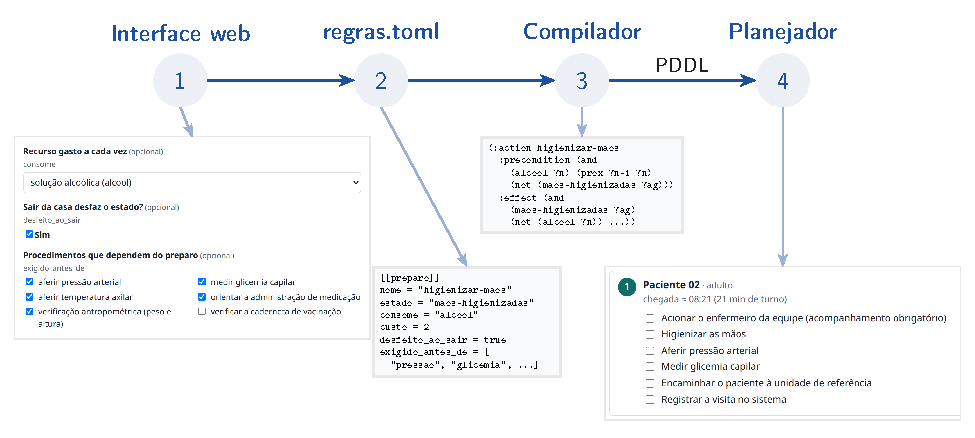
\includegraphics[width=\textwidth]{figs/01-compilador.pdf}
\end{frame}

% 5 — Os cinco modelos, com um exemplo cada.
\newcommand{\modelo}[3]{\caixaalta{#1}{22mm}{{\large\color{blue}#2\par}\vspace{1.5mm}#3}}
\begin{frame}{Cinco modelos fixos}
  \centering
  \modelo{.28\textwidth}{A. Recurso}{6 doses de álcool por saída, repostas na UBS.}\hfill
  \modelo{.28\textwidth}{B. Preparo}{Higienizar as mãos, gastando uma dose.}\hfill
  \modelo{.28\textwidth}{C. Pré-requisito}{Higienizar antes de aferir a pressão.}\par
  \vspace{5mm}
  \modelo{.40\textwidth}{D. Consumo}{Cada glicemia gasta 2 bolas de algodão.}\hspace{6mm}
  \modelo{.40\textwidth}{E. Exigência por paciente}{Suspeita de tuberculose exige N95 para iniciar a visita.}\par
\end{frame}

\section{Na prática}
% 6 — A interface: um formulário por modelo.
\begin{frame}{Escrevendo uma regra}
  \centering
  {\large O formulário do modelo preparo para Higienizar as mãos\par}
  \vspace{4mm}
  \captura{width=.72\textwidth}{figs/capturas/regras-formulario-trecho.png}
\end{frame}

% 7 — Cada campo e conferido enquanto se digita.
\begin{frame}{Conferido enquanto se digita}
  \centering
  {\large O erro vem com a correção.\par}
  \vspace{6mm}
  \captura{width=.92\textwidth}{figs/capturas/regras-sugestao.png}\par
  \vspace{4mm}
  {\large Com tudo válido, a equipe baixa o \texttt{regras.toml}.\par}
\end{frame}

% 8 — O resultado para o ACS: roteiro e mapa.
\begin{frame}{O roteiro e a rota}
  \begin{columns}[T,onlytextwidth]
    \column{.52\textwidth}
    {\large\color{blue}Roteiro\par}
    \vspace{2mm}
    \captura{width=.98\textwidth}{figs/capturas/roteiro-visita.png}
    \column{.45\textwidth}
    {\large\color{blue}Rota\par}
    \vspace{2mm}
    \captura{width=.98\textwidth}{figs/capturas/mapa.jpg}
  \end{columns}
\end{frame}

% 10 — O roteiro impresso, numa folha A4 (impressao do proprio navegador).
\begin{frame}{O roteiro pode ser impresso}
  \begin{columns}[c,onlytextwidth]
    \column{.42\textwidth}
    {\large Uma folha por turno, com caixas para marcar cada tarefa.\par}
    \column{.54\textwidth}
    \centering
    \folha{height=.8\textheight}{figs/capturas/roteiro-impresso.pdf}
  \end{columns}
\end{frame}

\section{Resultados}
% 11 — Avaliação: três resultados, em cartões com faixa de título.
\newcommand{\resultado}[3]{%
  \begin{tikzpicture}[baseline=0pt]       % alinhados pelo topo
    \def\L{4.25cm}\def\A{4.6cm}
    \draw[draw=blue!40,fill=blue!5,rounded corners=4pt] (0,0) rectangle (\L,-\A);
    \fill[blue,rounded corners=4pt] (0,0) rectangle (\L,-9mm);
    \fill[blue] (0,-5mm) rectangle (\L,-9mm);
    \node[text=white,font=\large\bfseries] at (.5*\L,-4.5mm) {#1};
    \node[anchor=north,text width=\L-8mm,align=center] at (.5*\L,-14mm)
      {{\Large\bfseries\color{blue}#2\par}\vspace{3mm}
       {\color{muted}\rule{12mm}{.6pt}\par}\vspace{2mm}
       {\small #3}};
  \end{tikzpicture}}
\begin{frame}{O que medimos}
  \centering
  \resultado{Mais curto}{7 a 18 linhas}{de TOML por regra, contra 13 a 60 linhas de PDDL
    alteradas}\hfill
  \resultado{Barato}{+1 a 9 min}{por regra, num turno ótimo de 386 min}\hfill
  \resultado{Escala}{30 s}{para 7 regras e 10 pacientes, com o Fast Downward}\par
  \vspace{5mm}
  \muted{Regras e pacientes sintéticos, não normas nem dados reais.}
\end{frame}

\section{Próximos passos}
% 10 — Limites honestos e o que vem a seguir.
\begin{frame}{Limites e próximos passos}
  \begin{columns}[T,onlytextwidth]
    \column{.48\textwidth}
    \centering
    {\large\color{blue}Ainda fora dos modelos\par}
    \vspace{4mm}
    \caixaalta{.86\textwidth}{17mm}{\textbf{Alternativas}\\Higienizar as mãos \emph{ou} usar luvas}\par
    \vspace{2mm}
    \caixaalta{.86\textwidth}{17mm}{\textbf{Horário do dia}\\Visitar gestantes pela manhã}\par
    \column{.48\textwidth}
    \centering
    {\large\color{blue}Próximos passos\par}
    \vspace{4mm}
    \caixaalta{.86\textwidth}{17mm}{\textbf{Usabilidade}\\Teste com quem não programa}\par
  \end{columns}
\end{frame}

% Créditos, como na semana 1.
\begin{frame}{Encerramento e créditos}
  \centering
  {\large Obrigado pela participação!\par}
  \vspace{9mm}
  \begin{columns}[T,onlytextwidth]
    \column{.48\textwidth}
    \centering
    {\large\color{blue}Projeto original\par}
    \vspace{2mm}
    \textbf{Grupo B -- Ciclo 2}\par
    \vspace{4mm}
    Gabriel Knopp\par
    Arthur Silva\par
    Izadora Oliveira
    \column{.48\textwidth}
    \centering
    {\large\color{blue}Compilador e interface\par}
    \vspace{2mm}
    \textbf{Grupo B -- Ciclo 3}\par
    \vspace{4mm}
    Luis Junior\par
    Manuela Dalmonte\par
    Vítor Feijó
  \end{columns}
\end{frame}

\end{document}
